\documentclass{ctexart}
\usepackage{EC}
\begin{document}
\section{碳及其化合物}
\subsection{单质碳}
\subsubsection{石墨}
\paragraph{石墨的结构,性质与反应}
众所周知,石墨具有六边形\ce{\{C6\}}环稠合的二维层状结构.
\chemfig{graphite-1}{1}{石墨的二维层状结构示意图}
根据层间重叠方式的不同,石墨有两种异构体,即六方$\alpha$-石墨和三方$\beta$-石墨,前者在自然界中占据主要(约$70\%$).两者的晶体结构如下所示.
\bichemfig{alpha-graphite}{1}{六方$\alpha$-石墨的晶体结构示意图}{beta-graphite}{1}{三方$\beta$-石墨的晶体结构示意图}{石墨的两种异构体(黑点表示碳原子,虚线表示晶胞边界)}
从密堆积的角度描述这两种石墨的结构,六方$\alpha$-石墨的堆积层可以表示为$\cdots AB\overline{AB}AB\cdots$,而三方$\beta$-石墨的堆积层可以表示为$\cdots ABC\overline{ABC}ABC\cdots$.研磨$\alpha$-石墨可以使其转化为$\beta$-石墨,而加热$\beta$-石墨可以使其转化为$\alpha$-石墨.不完全的转化将得到湍层石墨,其中各层的堆积次序是随机的.\\
\indent 由于每一层均可以视作无限稠合的芳环,因而电子在层内是高度离域的,这使得石墨具有良好的导电性能,并且平行于层方向的电导率大约是垂直于层方向的$10^3$倍.\\
\indent 石墨的层间间距较大,只有不强的范德华力作用,使得其容易沿层平面滑动解理\footnote{\tbf{解理}(cleavage)又称\tbf{劈理},是矿物学和宝石学的常见术语,指的是矿物或宝石晶体在外力的作用下,沿一定的结晶学方向裂开成光滑平面的性质.这些光滑平面被称为\tbf{解理面}或\tbf{劈理面}.}.因此,石墨的硬度很低.\\
\indent 石墨的独特的层状结构使得它与\ce{F2}反应时控制条件就能形成理想化学式为\ce{CF}的分子.这种分子由无限延伸的椅式六元环稠合而成,所有\ce{F}原子分居平面两侧.
\paragraph{石墨的分布,生产与用途}
晶状的石墨广泛分布于全世界,然而大多数以薄片的形式存在于硅酸盐矿石中,几乎没有经济价值.由于缺乏天然的来源,石墨在工业上主要通过焦炭与二氧化硅的反应制备:
\begin{center}
    \ce{SiO2 + 3C -> SiC}\\
    \ce{SiC(s) ->T[$2500\tc$] Si(g) + C(s,\text{石墨})}
\end{center}
石墨的主要用途如下:
\begin{enumerate}[label=\tbf{\arabic*.},topsep=0pt,parsep=0pt,itemsep=0pt,partopsep=0pt]
    \item \tbf{作为铅芯的主要成分制造铅笔}\\
        石墨的层状结构易剥落,可用于纸上书写.现代铅笔笔芯以石墨和黏土制造,石墨含量越高,铅芯越软,颜色越黑.\\
        铅笔之名源自其早期雏形为铅金属所制造,而后则又因欧洲中世纪时石墨被误以为是铅的一种,而有了\tbf{黑铅}这个名称,因此铅笔一词在各语言中流传使用而未修正.中国古代的铅笔事实上确为铅粉所制,并没有石墨.
    \item \tbf{惰性电极材料}\\
        石墨的优良的导电性和稳定性使得其可以作为电极材料.这一方案显然比铂电极更加便宜,并且不会受到卤素的侵蚀.因此,电解\ce{NaCl}水溶液制备\ce{Cl2}和\ce{NaOH}时通常采用石墨电极.
    \item \tbf{核反应堆的中子减速剂}
        石墨可以有效地减缓核反应堆里中子的速度,有效控制反应进行.石墨耐高温,纯度高,是迄今为止核反应堆中极为重要的原材料.
\end{enumerate}
\subsubsection{金刚石与蓝丝黛尔石}
\paragraph{金刚石的结构与性质}
在金刚石中,\ce{C}原子以$\text{sp}^3$杂化形式与相邻的\ce{C}原子成键,从而形成无限延伸的三维结构.金刚石也有两种异构体.大多数天然得到的或人工合成的金刚石均属立方晶系,因此一般而言我们所称的金刚石为立方金刚石.1967年在美国亚利桑那州的巴林杰陨石坑第一次鉴别出了六方金刚石,并以爱尔兰晶体学家D. K. Lonsdale\footnote{1929年, D. K. Lonsdale首次利用X射线衍射法证明了苯是平面的.1931年,她又首次利用Fourier变换光谱分析法解析了六氯苯的结构,为推动芳香性的研究做出了重大贡献.她是英国皇家化学会首次选入的两个女会士之一,伦敦学院大学的首位终身女教授,国际晶体学会第一位女主席,英国科学促迸学会首位女主席.}命名为蓝丝黛尔石.两者的结构如下所示.
\bichemfig{diamond-1}{0.1}{立方金刚石的晶体结构}{diamond-2}{0.1}{六方金刚石的晶体结构}{两种金刚石的晶体结构}
事实上,分别将闪锌矿和纤锌矿中的所有原子替换为碳原子即可分别得到立方金刚石和六方金刚石.\\
\indent 蓝丝黛尔石推测为流星上的石墨坠入地球时在高温高压下形成.它保留了石墨的平行六边形结构,但层间的碳原子成键.蓝丝黛尔石相较立方金刚石不稳定,这可能是因为其中存在船式六元环(即存在重叠式构象的碳原子)所致.有研究表明,蓝丝黛尔石具有比立方金刚石更高的硬度和更强的抗压能力.然而,天然存在的蓝丝黛尔石不纯,且并不完全为六方结构.\\
\indent 金刚石是已知硬度最高的天然物质.同时,它的化学性质也非常稳定,即使在纯\ce{O2}中也要加热到$720\tc$才能燃烧.
\paragraph{金刚石的合成与应用}
由于金刚石的硬度极高且导热性极高,因此常用于用于钻探,研磨工具之上,可以用来切削和刻划其他物质.自1955年通用电气发明通过高温高压处理石墨获得人造金刚石的技术以来,人们已经可以利用气相沉积法等制成金刚石微粒,因此现在细小颗粒的人工合成钻石已经较同级天然钻石便宜.故此,天然钻石的工业价值已经完全消失,目前的主要用途已仅限于首饰与观赏.随着人工合成技术的成熟,合成钻石也进入了首饰市场,但总是遭到天然钻石公司的诋毁.
\subsubsection{石墨烯}
\paragraph{石墨烯的结构与性质}
石墨烯又称单层石墨,碳单层,是由石墨剥层制造出的碳单质.石墨烯的碳原子以$\text{sp}2$杂化轨道组成六角型呈蜂巢晶格的单层平面薄膜,其厚度仅相当于1个碳原子的直径.\\
\indent 石墨烯几乎是完全透明的,它的透光率为$97.7\%$.与石墨类似的,它具有极高的导热和导电性能.
\paragraph{石墨烯的制备与应用}
2004年,曼彻斯特大学和俄国切尔诺戈洛夫卡微电子工艺研究所的两组物理团队共同合作,首先分离出单独石墨烯平面.海姆和团队成员偶然地发现了一种简单易行的制备石墨烯的新方法,他们将石墨片放置在塑料胶带中,折叠胶带粘住石墨薄片的两侧.撕开胶带,薄片也随之一分为二.不断重复这一过程,就可以得到越来越薄的石墨薄片,而其中部分样品仅由一层碳原子构成,这就制得了石墨烯.\\
\indent 除此之外,还可以采用在\ce{Ni}基底上进行气相沉积法等方法.总之,由于石墨烯的广泛的潜在用途,人们仍然在对改进工艺,提高制备效率和纯度等方面进行努力.\\
\indent 石墨烯凭借其超凡的导电性,导热性,机械强度,柔韧性和透明度,在众多领域展现出革命性的应用潜力.在电子领域,它是制造超快芯片,柔性透明电极(用于可折叠屏幕和触摸屏)的理想材料;在能源领域,它能显著提升锂电池,超级电容器的充放电速度和容量,并用于高效太阳能电池;在材料领域,它用于制造更轻,更强,更耐用的复合材料和防腐,导电,导热涂层;此外,它在高灵敏度传感器,高效海水淡化膜,水处理过滤膜,生物医学(如药物递送,生物传感)以及可穿戴技术等方面也具有广阔前景,被视为推动未来科技发展的关键材料之一.
\subsubsection{石墨炔}
\subsubsection{富勒烯及其衍生物}
\paragraph{富勒烯的制备}
富勒烯又称球碳,是由纯碳原子组成的球形分子.这类分子可以通过在石墨电极间放电后形成的碳烟中分离得到,也可以在严格控制下使苯不完全燃烧,在形成的碳烟中分离得到.
\paragraph{足球烯的结构与反应}
1985年英国化学家哈罗德·沃特尔·克罗托博士和美国科学家理查德·斯莫利在莱斯大学制备出了第一种富勒烯,即\tbf{足球烯}\ce{C_60}.它的骨架结构与足球一致,属于$I_{\text h}$点群,具有很高的对称性,同时也是最常见和最稳定的富勒烯.
\begin{figure}[H]
    \centering
    \subfigure[\ce{C60}的结构]{
        \centering\begin{minipage}[b]{.3\linewidth}
            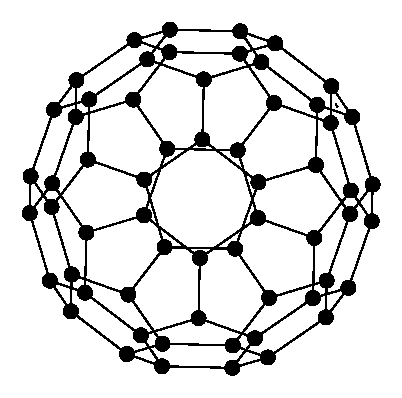
\includegraphics[scale=0.75]{picture/C60-1.eps}
        \end{minipage}
    }
    \subfigure[\ce{C60}的成键方式示意图]{
        \centering\begin{minipage}[b]{.3\linewidth}
            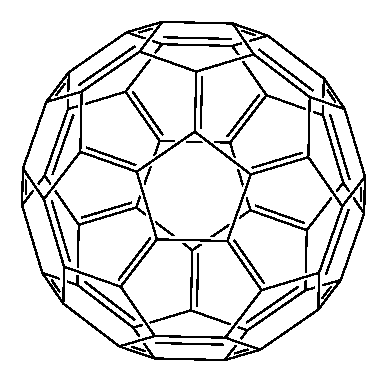
\includegraphics[scale=0.75]{picture/C60-2.eps}
        \end{minipage}
    }
    \subfigure[\ce{C60}的平面示意图]{
        \centering\begin{minipage}[b]{.3\linewidth}
            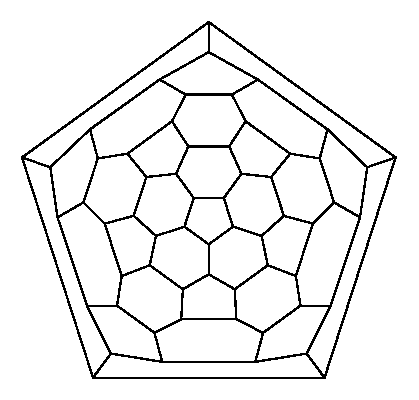
\includegraphics[scale=0.75]{picture/C60-3.eps}
        \end{minipage}
    }\vspace{-10pt}\caption{\ce{C60}分子的结构}
\end{figure}
\ce{C60}一共有12个五边形面和20个六边形面,其中每个五元环都与五个六元环相接,而每个六元环都与三个五元环和三个六元环交替相接.不难看出,\ce{C60}中的所有\ce{C}原子均等价.
\paragraph{\ce{C60}的体积}
\ce{C60}中两个六元环共用\ce{C-C}键的键长为$138.8\text{ pm}$,五元环和六元环共用\ce{C-C}键的键长为$143.2\text{ pm}$.根据键长数据,我们可以求出\ce{C60}分子的体积\footnote{当然,我们可以用内切球,外接球等方法近似计算其体积.这里采取精确计算的办法.}.\\
\indent 不难看出,\ce{C60}的结构与三角二十面体有很大的相似性.为此,我们可以把所有两个六元环共用的边延长,将\ce{C60}补全为一个正三角二十面体.这一过程的逆过程即在三角二十面体的每个顶点截去一个正五棱锥.由于原来的三角二十面体的每个面都是正三角形,因此截面的五边形的边长与五棱锥的棱长相等.因此,这个正三角二十面体的边长为
\[a=d_{66}+2d_{56}=(138.8+143.3\times2)\text{pm}=425.2\text{ pm}\]
经过三角二十面体的对棱(不妨记为$A_1A_2$和$A_3A_4$)取截面,那么$A_1A_2A_3A_4$应当是一个矩形,矩形的中心$O$即为三角二十面体的中心.短边长度$d_1=a=425.2\text{ pm}$,长边即五边形对角线,其长度
\[d_2=\sqrt{2a^2\left(1-\cos108^\circ\right)}=688.0\text{ pm}\]
于是中心$O$到顶点$A$的距离为
\[r=\dfrac{\sqrt{d_1^2+d_2^2}}{2}=404.4\text{ pm}\]
取任意三角形面的面心$B$,中心$O$到$B$的距离为
\[h_1=\sqrt{r^2-\left(\dfrac{\sqrt3}{3}a\right)^2}=321.3\text{ pm}\]
于是该三角二十面体的体积为
\[V_1=20\cdot\dfrac13\cdot\dfrac{\sqrt3}{4}a^2h_1=1.677\times10^{8}\text{ pm}^3\]
\indent 现在我们计算截去的五棱锥的体积.五棱锥的高为
\[h_2=\sqrt{d_{56}^2-\left(\dfrac{d_{56}}{2\cos54^\circ}\right)^2}=75.28\text{ pm}\]
于是五棱锥的体积为
\[V_2=\dfrac13\cdot\left(5\cdot\dfrac12\cdot d_{56}\cdot\dfrac{\tan54^\circ d_{56}}{2}\right)\cdot h_2=8.854\times10^5\text{ pm}^3\]
\indent 对于\ce{C60}而言,一共截去了$12$个五棱锥,因此\ce{C60}的体积为
\[V=V_1-12V_2=1.571\times10^{8}\text{ pm}^3\]
\indent 这是一道锻炼空间想象和立体几何能力的题目.你还可以采取其它计算方法得到它的体积.
\paragraph{\ce{C60}中碳的杂化形式}
在探讨这一问题之前,我们需要了解一些关于杂化的知识.$\text{sp}^i$杂化的轨道的波函数为
\[\psi_{\text{sp}^i}=a\phi_{\text s}+b_x\phi_{\text{p}_x}+b_y\phi_{\text{p}_y}+b_z\phi_{\text{p}_z}\]
其中$\phi_{\text s}$和$\phi_{\text{p}_x},\phi_{\text{p}_y},\phi_{\text{p}_z}$分别为$s$轨道和三个$p$轨道的波函数.为了方便考虑,我们最好让$\text{p}$轨道归一化.令
\[b=\sqrt{b_x^2+b_y^2+b_z^2}\ \ \ \ \ \phi_{p}=\dfrac{b_x\phi_{\text{p}_x}+b_y\phi_{\text{p}_y}+b_z\phi_{\text{p}_z}}{\sqrt{b_x^2+b_y^2+b_z^2}}\]
你可以将$\phi_{\text{p}_x},\phi_{\text{p}_y},\phi_{\text{p}_z}$分别视作空间中三个方向上的单位向量,上述过程实际上是求出三个$\text p$轨道线性组合后指向方向的单位向量,这就是归一化$\text p$轨道的意义.由于$\text{s}$轨道并无特殊取向,因此$\text{sp}^i$杂化的轨道取向由$\phi_p$的取向决定.\\
\indent 现在再来考虑组合后的波函数本身应当满足的性质:归一性和正交性.为了方便,下面就用向量的形式表示函数.对于轨道$\phi_{\text{sp}^i}$,归一性要求
\[a^2+b^2=1\]
现在考虑两个$\phi_{\text{sp}^i}$轨道,将它们分别表示为
\[\overrightarrow{\psi_{\text{sp}^i_A}}=a\overrightarrow{\phi_{\text{s}}}+b\overrightarrow{\phi_{\text{p}_A}}\ \ \ \ \ \overrightarrow{\psi_{\text{sp}^i_B}}=a\overrightarrow{\phi_{\text{s}}}+b\overrightarrow{\phi_{\text{p}_B}}\]
它们之间的夹角,即键角为$\theta$,这意味着决定两者方向的$p$轨道函数的夹角为$\theta$.正交性要求
\[\overrightarrow{\psi_{\text{sp}^i_A}}\cdot\overrightarrow{\psi_{\text{sp}^i_B}}=0\]
由于$s$轨道和任意方向上的$p$轨道都是正交的,于是$\overrightarrow{\phi_{\text{s}}}\cdot\overrightarrow{\phi_{\text{p}}}=0$.于是上式即为
\[a^2+b^2\overrightarrow{\phi_{\text{p}_A}}\cdot\overrightarrow{\phi_{\text{p}_B}}=0\]
我们说过,$\overrightarrow{\phi_{\text{p}}}$的几何意义为指向空间中某一方向的单位向量,那么两个夹角为$\theta$的单位向量的内积显然应当是$\cos\theta$.于是就有
\[a^2+b^2\cos\theta=0\]
将归一化条件代入其中就有
\[a^2=-\dfrac{\cos\theta}{1-\cos\theta}\ \ \ \ \ b^2=\dfrac{1}{1-\cos\theta}\]
采取$\text{sp}^i$意味着$\text{s}$轨道和$\text{p}$轨道的比例为$1:i$,这可以用线性组合系数的平方之比来表示,这样就有
\[i=\dfrac{b^2}{a^2}\]
结合上面的式子就有
\[1+i\cos\theta=0\]
或者
\[\theta=\arccos\left(-\dfrac1i\right)\]
这样,你就可以计算各种$\text{sp}^i$杂化中$i$的具体数值,例如\ce{H2O}中的\ce{O}接近$\text{sp}^4$杂化.\\
\indent 对于\ce{C60}而言,我们可以近似地采取平均键角进行计算.每一个碳都被两个六边形和一个五边形所共用,平均键角
\[\overline{\theta}=\dfrac{108^\circ+2\times120^\circ}{3}=116^\circ\]
于是杂化指数
\[i=-\dfrac{1}{\cos116^\circ}=2.28\]
这就是\ce{C60}中的\ce{C}原子采取$\text{sp}^{2.28}$杂化的由来.
\paragraph{\ce{C60}的晶体结构}
正常情况下,\ce{C60}晶体属立方晶系,\ce{C60}分子按照立方最密堆积形成晶体.\\
\indent 说到这一晶体的结构,就不得不提到\ce{K3C60}这一化合物.其中\ce{K+}填入所有\ce{C60}形成的四面体空隙和八面体空隙.这一物质的有趣的一点是其中\ce{K}的质量分数为$14.000\%$\footnote{所谓蕉下客.}.
\paragraph{\ce{C60}的化学性质}
尽管结构中大量存在苯环,\ce{C60}的芳香性却并不像苯一样如此明显.从键长数据也可以看出,\ce{C60}中的双键更多时候趋向于定域化,这意味着它能发生与烯烃类似的反应.此外,大的共轭体系也使得其能被单电子氧化/还原.以下是一些反应的例子.
\begin{enumerate}[label=\tbf{\arabic*.},topsep=0pt,parsep=0pt,itemsep=0pt,partopsep=0pt]
    \item \tbf{加成反应}\\
        \ce{C60}能被各种手段加氢.Birch还原能将其还原为\ce{C60H32},用二氢化蒽能将其还原为\ce{C60H36},等等.然而,\ce{C60H60}却因为键角的缘故而难以得到.\\
        \ce{C60}也可以与卤素反应.与\ce{F2}的反应倾向于生成$1,2$位的二取代物,而与\ce{Cl2}和\ce{Br2}的反应倾向于加成到相距较远的\ce{C}原子上,例如\ce{C60Br8}和\ce{C60Br24}.\\
        \ce{C60}也可以与\ce{PhCN2}等卡宾前体反应生成含有三元环的\ce{C61Ph2}.它也可以自己发生$[2+2]$环加成反应二聚成为\ce{C120}.
    \item \tbf{氧化/还原反应}\\
        在合适的氧化剂存在下,可以形成\ce{C60^n+};在合适的还原剂存在下则可以形成\ce{C60^n-}.
\end{enumerate}
\paragraph{其它富勒烯}
除去最常见的\ce{C60}之外,还有\ce{C70},\ce{C84}等富勒烯分子.它们也是笼状结构的分子,但对称性并没有\ce{C60}高.
\subsubsection{碳纳米管}
\subsubsection{无定形碳}
\paragraph{无定形碳的分布}
碳在史前就被认为是一种物质(炭,烟灰),而学界承认碳是一种元素却是18世纪几个实验的结论.大部分无定形碳都含有石墨的层状结构,然而晶体化程度很低,没有固定形状和周期性结构规律,同时经常掺杂很多其它元素.
\paragraph{焦炭}
煤经过高温碳化产生的焦炭是一种石墨化程度很差的碳,其大多数用于高炉炼钢.
\paragraph{碳黑}
碳黑是由液体烃或天然气的不完全燃烧制得的.这种颗粒很小的碳单质主要用于橡胶工业以强化橡胶,也可以用于墨水,油漆,纸张和塑料中的颜料.
\paragraph{活性炭}
活性炭是是黑色粉末状或颗粒状的碳物质.活性炭在微观上的不规则排列使得其在交叉连接之间有细孔,在活化时会产生碳组织缺陷,因此它是一种多孔的物质,具有很大的比表面积.\\
\indent 正因如此,活性炭广泛地用于脱色剂(在蔗糖工业中),空气和水体精华以及催化剂载体.它本身也可以催化一些反应,例如\ce{CO}与\ce{Cl2}反应生成\ce{COCl2}等.
\subsection{碳化物}
和硼化物一样,碳化物的种类也十分繁多,且彼此之间似乎也难以有清晰的界限.这里主要分出几类分别进行介绍.
\subsubsection{石墨间充化合物}
石墨中互相平行的碳原子平面层之间的距离比较大,而且层间的主要作用力是较弱的范德华力,这使得大量物质在温和条件下可能插入平面问得到不同组分的片
状化合物.1926年,人们发现石墨与\ce{K}蒸汽在$300\tc$能直接反应形成青铜色的\ce{KC8},这是第一个被制备出的碱金属石墨化物.它的晶体结构示意如下:
\bichemfig{KC8-1}{0.1}{\ce{KC8}的晶体结构}{KC8-2}{0.75}{\ce{KC8}的层投影}{\ce{KC8}的结构}
\ce{KC8}中的石墨层的$c$轴投影相互重叠,两层石墨层间的\ce{K}原子按照上图的方式分布,然后依$\cdots ABCABC\cdots$的方式堆积形成三方晶系的晶体.\\
\indent 除了\ce{KC8}以外,还可以用碱金属制得\ce{MC12},\ce{MC24},\ce{MC36},\ce{MC48}和\ce{MC60}等化合物.它们的结构都以\ce{KC8}为基础,但金属层缺失了图5(b)中心的\ce{M}原子(相当于有规律地缺失了$\dfrac13$的\ce{M}原子),因而形成\ce{MC_{12n}}系列的化合物.如果每层石墨层间都有这样的金属层,即为\ce{MC12};相比\ce{MC12},金属层隔层出现即为\ce{MC24},依此类推.\\
\indent 碱土金属和过渡金属能形成\ce{MC6},其金属层的填充方式也如下所示.
\begin{figure}[H]
    \centering
    \subfigure[\ce{MC12}的结构及其与\ce{MC8}的联系]{
        \begin{minipage}[b]{.55\linewidth}
            \centering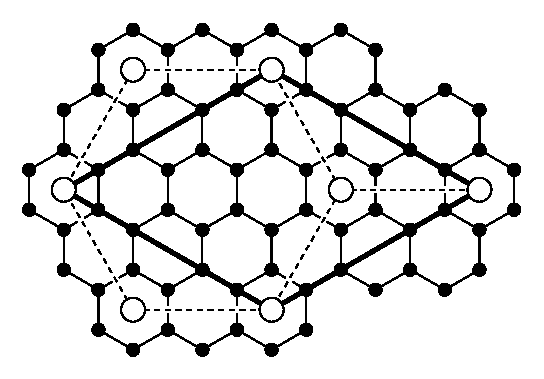
\includegraphics{picture/MC12.eps}
        \end{minipage}
    }
    \subfigure[\ce{MC6}的结构]{
        \begin{minipage}[b]{.35\linewidth}
            \centering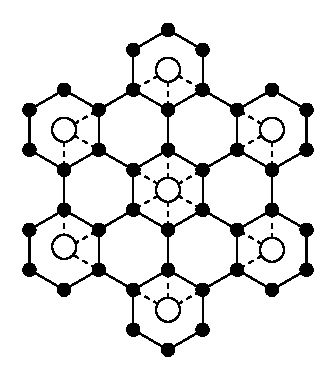
\includegraphics{picture/MC6.eps}
        \end{minipage}
    }
\end{figure}
这些金属石墨化物有着极高的电导率(大约是石墨的十倍)以及更鲜明的颜色.这意味着它们的本质应当是金属将电子转移至石墨层的导带而形成了二维层状阴离子,阳离子则镶嵌其中.\\
\indent 金属石墨化合物(尤其是碱金属石墨化合物)在空气中极为活泼,遇水可能发生爆炸.\ce{KC8}经常作为各类反应中的强还原剂而使用,尤其是制备各类低价金属配合物时.还原得到的\ce{C}单质以石墨的形式存在,容易处理.
\subsubsection{离子型碳化物}
\paragraph{似盐型碳化物}
某些碳化物中的碳显$-4$价,它们的水解产生\ce{CH4}.典型的此类化合物有\ce{Be2C}和\ce{Al4C3}.两者分别可以由如下的反应得到:
\begin{center}
    \ce{2BeO + 2C ->T[$2000\tc$] Be2C + CO}\\
    \ce{4Al + 3C ->T[高温] Al4C3}
\end{center}
前者具有反萤石型的结构.后者的结构则比较复杂,但其中的\ce{Al}与大多数情况相似,被\ce{C}原子四配位的.
\paragraph{含有\ce{C2}单元的碳化物}
这类碳化物是为人所熟知的,其中最著名的就是炔化钙\ce{CaC2}(通常称作\tbf{电石}).在工业上按照下面的方法制备\ce{CaC2}:
\begin{center}
    \ce{CaO + 3C ->T[$2200\sim2500^\tc$] CaC2 + CO}
\end{center}
在过去,\ce{CaC2}作为\ce{C2H2}的主要来源,现在则更多的来源于石油工业.\ce{CaC2}与水反应即生成乙炔,与\ce{N2}反应生成氰氨化钙,后者的水解生成氨基氰这一化肥工业的重要原料:
\begin{center}
    \ce{CaC2 + 2H2O -> C2H2 + Ca(OH)2}\\
    \ce{CaC2 + N2 ->T[$1000\sim1200^\tc$] CaCN2 + C}\\
    \ce{CaCN2 + 2H2O -> H2NCN + Ca(OH)2}
\end{center}
\ce{CaC2}是无色固体.常温下的\ce{CaC2}中\ce{CA^2+}与\ce{C_2^2-}按照\ce{NaCl}的形式排列,由于\ce{C2^2-}是线形阴离子而变为四方晶系.加热后的\ce{CaC2}则属于立方晶系,对称性的升高源自\ce{C_2^2-}排列方向的随机化,完全转变为\ce{NaCl}型.
\bichemfig{CaC2-1}{0.1}{常温下\ce{CaC2}的晶体结构}{CaC2-2}{0.1}{高温下\ce{CaC2}的晶体结构}{\ce{CaC2}的晶体结构}
与\ce{CaC2}类似的还有镧系元素形成的\ce{LnC2}和\ce{Ln4(C2)3}.与\ce{CaC2}不同,大多数\ce{LnC2}具有良好的导电性,这说明它们之中的\ce{Ln}应当以\ce{Ln^3+}的形式存在,多余的自由电子在\ce{C2^2-}的反键轨道上部分离域,因此其中的\ce{C-C}键的键长相较\ce{CaC2}明显更长.这也使得它们的水解产物比较复杂,经常有\ce{C2H4}等还原产物的生成.
\subsubsection{填隙型碳化物}
填隙碳化物是难溶的,极坚硬的,耐火的材料,并保持了许多金属的特性(例如具有金属光泽和很高的电导率),因此把它们作为合金看待似乎更加合适.这其中最典型的化合物是\tbf{渗碳体}\ce{Fe3C}.渗碳体是钢铁中最硬的相,是钢铁获得高强度,高硬度和耐磨性的基础.它具有复杂的晶体结构,属于正交晶系:
\chemfig{Fe3C}{0.12}{\ce{Fe3C}的晶体结构}
\subsection{碳的氧化物及碳酸盐}
碳形成两种稳定的,也是为人所熟知的氧化物,即\ce{CO}和\ce{CO2}.此外,还有一些不大稳定的氧化物,例如\ce{C3O2}等等.
\subsubsection{碳的复杂氧化物}
\paragraph{二氧化三碳\ce{C3O2}}
\ce{C3O2}的正式名称为1,2-丙二烯-1,3-二酮,是有腐败气味的气体,由丙二酸用\ce{P4O10}脱水得到.正如化学式所描述的那样,这一分子具有\ce{O=C=C=C=O}的线性结构.\ce{C3O2}容易发生聚合,形成六元环内酯并接的链状结构.
\chemfig{C3O2}{1}{\ce{C3O2}聚合后的结构}
\ce{C3O2}容易与\ce{H2O}发生反应再次形成丙二酸,与\ce{HCl}或\ce{NH3}反应则得到对应的酰氯和酰胺,因此可以将它视作丙二酸酐.
\paragraph{苯六酸酐\ce{C12O9}}
苯六酸酐又称蜜石酸酐,是苯六酸(即蜜石酸\footnote{这一名字来源于蜜蜡石\ce{Al2[C6(COO)6].16H2O}.})的酸酐,可以由苯六酸与酰氯或酸酐的反应得到:
\chemfig{C12O9-1}{1}{\ce{C12O9}的制备方式与结构}
从结构与性质上看,把它归为有机物似乎更合适,但它毕竟不含\ce{H}原子,因此放到氧化物一节稍作介绍.\\
关于苯六酸酐的另一个有趣的事实是用浓硫酸氧化石墨和足球烯等部分碳单质都能得到苯六酸酐,这可能是因为这些物质中本身就具有芳环结构.并且两者氧化的理论产率分别为$\dfrac67$和$\dfrac45$.这可以用下面的图来解释.
\bichemfig{C12O9-2}{0.9}{从石墨得到\ce{C12O9}}{C12O9-3}{0.8}{从\ce{C60}得到\ce{C12O9}}{由碳单质得到\ce{C12O9}的原子来源示意图}
\subsubsection{一氧化碳\ce{CO}}
\paragraph{\ce{CO}的结构}
我们都知道\ce{CO}是\ce{N2}的等电子体,键长为$112.8\text{ pm}$,相较普通的羰基(作为对比,\ce{HCHO}中的\ce{C=O}键键长为$120.8\text{ pm}$)长度更短,这意味着其中的键级应当大于$2$.\ce{CO}的极高的键能\footnote{似乎是已知共价键中键能最高的.}$1072\kJm$,以及较羰基明显更大的红外振动波数($2143\text{ cm}^{-1}$)也支持这一观点.理论计算的结果表明,\ce{CO}中的实际键级约为$2.6$.
\chemfig{CO-1}{1}{\ce{CO}的共振式}
尽管\ce{O}的电负性明显地大于\ce{C},但为了满足八电子结构,\ce{O}提供了一对电子额外形成$\pi$键,这也造成了\ce{CO}的偶极矩反常的小,并且事实上(正电荷指向负电荷)由\ce{O}指向\ce{C},这可以由上图右边的共振式的形式电荷反映出来.负电荷端在\ce{C}原子也意味着\ce{CO}在作为配体时几乎都用\ce{C}端作为配位原子.然而,当配位后,由于反馈$\pi$键的形成,负电荷端有时又回到\ce{O}上.\\
\indent \ce{CO}的基态是单线态,没有不成对的电子.
\paragraph{\ce{CO}的物理性质}
\ce{CO}是无色无味的剧毒气体,难溶于水,容易燃烧,有剧毒.
\paragraph{\ce{CO}的制备,化学性质与反应}
\ce{C}在有限量的氧气中或空气中直接氧化成\ce{CO},充足供氧时产生\ce{CO2}.温度较高时,\ce{CO2}倾向于分解生成\ce{CO},因此在高温或还原剂过量的情况下一般的产物均为\ce{CO}.
\subparagraph{\ce{CO}的工业制备与应用}
\ce{CO}以发生炉煤气或水煤气的形式广泛作为燃料使用.发生炉煤气由空气从红热的焦炭上通过得到,主要成分为\ce{CO}和\ce{N2},还含有少部分的\ce{CO2}和痕量的其它气体杂质.发生的反应为:
\begin{center}
    \ce{2C + O2 -> 2CO}\\
    \ce{C + O2 -> CO2}
\end{center}
水煤气则是将水蒸气从红热的焦炭上通过得到,其主要成分为\ce{CO}和\ce{H2}
\begin{center}
    \ce{C + H2O -> CO + H2}
\end{center}
\ce{CO}在工业上主要作为燃料和还原剂使用.关于其还原性,可以参考一般无机化学书上的Ellingham图以获取相关信息.
\subparagraph{\ce{CO}的实验室制备}
\indent 纯净的\ce{CO}可以用浓硫酸对甲酸或草酸脱水得到:
\begin{center}
    \ce{HCOOH ->T[浓硫酸] H2O + CO}\\
    \ce{H2C2O4 ->T[浓硫酸] H2O + CO + CO2}
\end{center}
然而\ce{CO}不能与水反应得到甲酸,因此不将其视作甲酸酐.\\
\indent 另外的方法包括加热锌粉与\ce{CaCO3}的混合物,或硝酸银与碘仿的反应:
\begin{center}
    \ce{Zn + CaCO3 -> ZnO + CaO + CO}\\
    \ce{CHI3 + 3AgNO3 + H2O -> 3HNO3 + CO + AgI}
\end{center}
\subparagraph{\ce{CO}的毒理学}
\ce{CO}可以与血红蛋白结合,结合的能力是\ce{O2}的$300$多倍,因此吸入\ce{CO}将抑制红细胞运输氧,致人失去知觉并死于窒息,这就是\ce{CO}的毒性来源.轻微的中毒可以通过呼吸新鲜空气解除,并且没有后遗症.频繁发生的室内\ce{CO}中毒案件通常是源于老旧的热水器或煤气灶的煤气泄漏,或是室内烧烤时不注意通风导致,并经常造成数人死亡的惨痛后果\footnote{为了您的健康,请使用天然气灶,电热水器,并且不在
再室内用炭炉烧烤.}.人们通常在煤气中添加诸如硫醚等具有明显气味的物质,以提醒使用者注意煤气泄漏.
\subparagraph{\ce{CO}的检测}
\ce{CO}能将水溶液中的\ce{PdCl2}还原成金属\ce{Pd},借由生成的黑色沉淀即可检验\ce{CO}.此法可能受到其它还原性气体的干扰.
\begin{center}
    \ce{CO + PdCl2 + H2O -> CO2 + 2HCl + Pd}
\end{center}
定量地测定\ce{CO}可以通过\ce{CuCl}的酸性溶液吸收形成加合物:
\begin{center}
    \ce{CuCl + CO + 2H2O -> Cu(CO)Cl(H2O)2}
\end{center}
\subparagraph{{\ce{CO}}的部分反应}
\ce{CO}在高温下与碱金属氢氧化物反应形成甲酸盐,与甲氧基化合物反应生成乙酸盐:
\begin{center}
    \ce{NaOH + CO -> HCOONa}\\
    \ce{MeONa + CO -> MeCOONa}
\end{center}

\indent \ce{CO}用碱金属的液氨溶液还原即可得到线性的\ce{C2O2^2-}.\\
\indent \ce{CO}和\ce{Cl2}或\ce{Br2}反应分别得到\ce{COCl2}或\ce{COBr2}.\ce{CO}与液态\ce{S}反应得到\ce{COS}.\\
\indent \ce{CO}与\ce{B2H6}在高压下反应得到对称的加合物\ce{H3BCO},但存在\ce{NaBH4/THF}时则生成环状的\ce{B3O3Me3}:
\begin{center}
    \ce{B2H6 + 2CO -> H3BCO}\\
    \ce{3B2H6 + 6CO -> 2B3O3Me3}
\end{center}
两者的结构如下所示.
\bichemfig{H3BCO}{1}{\ce{H3BCO}的结构}{B3O3Me3}{1}{\ce{B3O3Me3}的结构}{\ce{CO}与\ce{B2H6}的反应产物的结构}
\ce{CO}最重要的性质就是与过渡金属形成羰基化合物.这部分值得单独作为一个章节进行介绍,在这里就暂时略过.
\subsubsection{二氧化碳\ce{CO2}}
\paragraph{\ce{CO2}的物理性质}
\ce{CO2}是无色无味的气体,不可燃也不能助燃.\ce{CO2}可溶于水,但溶解度不大.固态的\ce{CO2}俗称\tbf{干冰},升华点为$-78\tc$\footnote{低温反应如果用干冰作为冷却剂,一般就会标注$-78\tc$,这在有机反应中很常见.}.
\paragraph{\ce{CO2}的制备与用途}
实验室制备\ce{CO2}可以用\ce{CaCO3}与稀\ce{HCl}反应得到:
\begin{center}
    \ce{CaCO3 + 2HCl -> CaCl2 + H2O + CO2}
\end{center}
工业上则是高温煅烧石灰石得到:
\begin{center}
    \ce{CaCO3 ->T[高温] CaO + CO2}
\end{center}
可以借由下面的两种方法实现\ce{CO2}的可逆回收与释放:
\begin{center}
    \ce{Na2CO3 + H2O + CO2 <=>T[冷却][加热] 2NaHCO3}\\
    \ce{2HO(CH2)2NH2 + H2O + CO2 <=>T[$25\sim65\tc$][$100\sim150\tc$] [HO(CH2)2NH3]2CO3}
\end{center}
有时,制备得到的\ce{CO2}中含有\ce{H2S}杂志,这可以通过近中性缓冲的\ce{KMnO4}的饱和溶液去除:
\begin{center}
    \ce{3H2S + 2KMnO4 + 2CO2 -> 3S + 2MnO2 + 2KHCO3 + 2H2O}
\end{center}

\indent \ce{CO2}最广泛的用途是作为冷冻剂.干冰主要用作冰淇淋,肉类和冷冻食品的致冷剂,并且用作一种方便的实验室冷冻剂和致冷剂.另一个主要用途是生产碳酸饮料\footnote{需要注意的是,碳酸饮料的酸性主要是其中添加的磷酸实现的.}.\ce{CO2}作为酸性气体可以中和碱性废水,也可以制造尿素:
\begin{center}
    \ce{CO2 + 2NH3 -> NH2COONH4}\\
    \ce{NH2COONH4 -> CO(NH2)2 + H2O}
\end{center}
\paragraph{\ce{CO2}的化学性质}
一般情况下,\ce{CO2}是含碳物质燃烧的最终产物.在较高的温度下,它会分解生成\ce{CO},因此高温反应一般不以\ce{CO2}作为产物写入方程式中.\\
\indent \ce{CO2}与格氏试剂\ce{RMgX}反应生成多一个碳的羧酸:
\begin{center}
    \ce{RMgX + CO2 -> RCOOMgX}
\end{center}

\indent 此外的最主要的性质就是\ce{CO2}的水溶液化学.我们单独将其写为一段.
\paragraph{\ce{CO2}的水溶液化学}
前面已经说过,\ce{CO2}可溶于水.溶于水的部分\ce{CO2}能与\ce{H2O}反应生成\ce{H2CO3}:
\begin{center}
    \ce{CO2(aq) + H2O(l) <=> H2CO3(aq)}\ \ \ $\dfrac{1}{K}=6\times10^2$
\end{center}
关于碳酸的性质,我们放在下一节描述.
\subsubsection{碳酸与碳酸盐}
\paragraph{\ce{H2CO3}的水溶液化学}
众所周知,碳酸\ce{H2CO3}是二元弱酸,两级电离平衡分别为
\begin{center}
    \ce{H2CO3(aq) + H2O(l) <=> H3O+(aq) + HCO3-(aq)}\\
    \ce{HCO3-(aq) + H2O(l) <=> H3O+(aq) + CO3^2-(aq)}
\end{center}
一般而言,碳酸的$K_{\text a1}$中的\ce{[H2CO3]}项是溶解的\ce{CO2}与\ce{H2CO3}的浓度之和.因此,碳酸的第一级表观电离常数和实际的电离常数分别为
\[K_{\text{a}1,\text{obs}}=\dfrac{\con{H3O+}\con{HCO3-}}{\con{CO2}+\con{H2CO3}}=4.45\times10^{-7}\]
\[K_{\text a1}=\dfrac{\con{H3O+}\con{HCO3-}}{\con{H2CO3}}=3.23\times10^{-4}\]
后面的数值就比较符合Pauling的预测了.第二级电离常数是可以测准的,为
\[K_{\text a2}=\dfrac{\con{H3O+}\con{CO3^2-}}{\con{HCO3-}}=4.84\times10^{-11}\]
\ce{H2CO3/HCO3-}缓冲对对于维持人体内环境的稳定有着举足轻重的作用,在自然界中也可以维持水体pH相对稳定.血浆的pH通常在$7.35\sim7.45$之间,因此人体的血液呈现弱碱性\footnote{一直以来有很多所谓人体是酸性还是碱性的说法,笔者认为有一定胡扯的成分.}.
\paragraph{高压碳酸盐化学}
在$20\text{ GPa}$的高压下加热\ce{SrO}与\ce{SrCO3}的混合物得到反钙钛矿型的\ce{Sr3CO5}:
\begin{center}
    \ce{2SrO + SrCO3 ->T[激光加热] Sr3CO5}
\end{center}
实际组成为\ce{[Sr^2+]3[CO4^4-][CO3^2-]},\ce{[CO4]^4-}占据(钙钛矿中,下同)\ce{Ca^2+}的位置,\ce{O^2-}占据\ce{Ti^4+}的位置,\ce{Sr^2+}占据\ce{O^2-}的位置.\\
\indent 在$82\sim138\text{ GPa}$的高压下,\ce{MgCO3}中的\ce{CO3^2-}发生三聚,形成六元环状的\ce{[C3O9]^6-}.\\
\indent 在$30\sim40\text{ GPa}$的高压下,用激光加热$\ce{MCO3}(\ce{M}=\ce{Ca},\ce{Sr})$和干冰的混合物可以得到\ce{MC2O5}.在\ce{CaC2O5}中存在与\ce{P4O10}结构相同的四聚离子\ce{[C4O10]^4-},而\ce{SrC2O5}中存在与\ce{N2O5}结构相同的\ce{[C2O5]^2-}.\\
\indent 以上提到的离子结构如下所示.
\begin{figure}[H]
    \centering
    \subfigure[\ce{[CO4]^4-}的结构]{
        \begin{minipage}[b]{.34\linewidth}
            \centering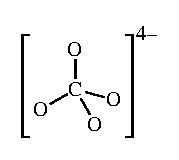
\includegraphics{picture/CO4^4-.eps}
        \end{minipage}
    }
    \subfigure[\ce{[C3O9]^6-}的结构]{
        \begin{minipage}[b]{.34\linewidth}
            \centering\includegraphics{picture/C3O96-.eps}
        \end{minipage}
    }
    \subfigure[\ce{[C4O10]^4-}的结构]{
        \begin{minipage}[b]{.34\linewidth}
            \centering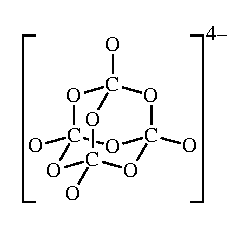
\includegraphics{picture/C4O104-.eps}
        \end{minipage}
    }
    \subfigure[\ce{[C2O5]^2-}的结构]{
        \begin{minipage}[b]{.34\linewidth}
            \centering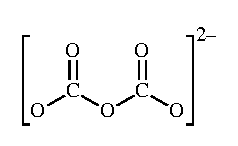
\includegraphics{picture/C2O52-.eps}
        \end{minipage}
    }\caption{高压下的碳酸根阴离子的结构}
\end{figure}
\subsubsection{碳的其它含氧酸及其盐}
\paragraph{草酸和草酸盐}
\paragraph{甲酸}
\subsection{碳的氢化物,卤化物和卤氧化物}
\subsection{碳的硫化物及其衍生物}
\subsubsection{碳的低硫化物}
\paragraph{一硫化碳\ce{CS}}
与\ce{CO}不同,\ce{CS}是一种非常不稳定的物质,几乎只能作为反应中间体存在.它容易与其它VIA族元素和卤素反应生成\ce{CSSe},\ce{CSTe},\ce{CSX2}等物质.\\
\indent 在光照下,\ce{CS2}发生\ce{C=S}键的解离生成\ce{CS}.当\ce{CS}浓度较大时,它会先二聚形成\ce{S=C=C=S},然后聚合形成\ce{(CS)_n}.这种聚合物具有如下两种可能的结构.
\bichemfig{(CS)n-1}{1}{\ce{(CS)_n}的可能结构I}{(CS)n-2}{1}{\ce{(CS)_n}的可能结构II}{\ce{(CS)_n}的结构}
\paragraph{三硫化二碳\ce{C3S2}}
对\ce{CS2}液体放电即可得到红色的液体\ce{C3S2},它像\ce{C3O2}那样也容易在室温下发生缓慢的聚合反应,并且产物的结构是类似的.
\subsubsection{二硫化碳\ce{CS2}}
\ce{C}的最重要的硫化物就是\ce{CS2}.
\paragraph{\ce{CS2}的物理性质}
\ce{CS2}是无色有毒液体,纯的\ce{CS2}有类似\ce{CHCl3}的芳香甜味,但是通常不纯的工业品因为混有其他硫化物(如\ce{COS})而变为微黄色,并且有令人不愉快的烂萝卜味.\\
\indent \ce{CS2}是良好的溶剂,可溶解硫单质或白磷.它本身在水中可溶,但溶解度并不大,$20\tc$时为$2.17\text{ g/L}$.
\paragraph{\ce{CS2}的制备}
过去,\ce{CS2}由硫蒸气和焦炭直接反应得到:
\begin{center}
    \ce{C + 2S ->T[$800\sim1000\tc$] CS2}
\end{center}
现在则主要通过天然气与硫蒸气的反应得到:
\begin{center}
    \ce{CH4 + 4S ->T[$600\tc$][\ce{SiO2/Al2O3}] CS2 + 2H2S}
\end{center}
这一反应类似甲烷在空气中的燃烧.
\paragraph{\ce{CS2}的性质,反应和用途}
在高压下,\ce{CS2}可以聚合形成链状的\ce{(CS2)_n},其中的\ce{C}为平面三角形配位:
\chemfig{(CS2)n}{1}{\ce{CS2}在高压下形成的链状聚合物}
\indent \ce{CS2}虽然在水中的溶解度不大,但可以与碱的溶液反应生成碳酸盐和硫代碳酸盐的混合物:
\begin{center}
    \ce{3CS2 + 6NaOH -> Na2CO3 + 2Na2CS3 + 3H2O}
\end{center}
\ce{CS2}也可以直接溶于含\ce{S^2-}的溶液中形成\ce{[CS3]^2-}:
\begin{center}
    \ce{CS2 + Na2S -> Na2CS3}
\end{center}

\indent 和\ce{CO2}类似,它与\ce{NH3}反应得到双硫代氨基甲酸铵,在\ce{Al2O3}存在时则生成硫氰酸铵\ce{NH4NCS},后者在加热时亦可转化为硫脲\ce{CS(NH2)2}:
\begin{center}
    \ce{CS2 + 2NH3 -> [NH4][H2NCS2]}\\
    \ce{CS2 + 2NH3 ->T[\ce{Al2O3}] NH4SCN + H2S}\\
    \ce{NH4SCN ->T[$160\tc$] CS(NH2)2}
\end{center}
类似地,\ce{CS2}与\ce{HNEt2}在\ce{NaOH}的水溶液中反应可以得到\ce{Et2NCS2Na},它可以作为市售无水乙醚的防爆剂:
\begin{center}
    \ce{NaOH + HNEt2 + CS2 -> Et2NCS2Na + H2O}
\end{center}

\indent \ce{CS2}与\ce{H2O}只能勉强地反应,在$200\tc$生成\ce{H2S}和\ce{COS},在更高温度下则生成\ce{H2S}和\ce{CO2},许多其它含氧化合物都可以与\ce{CS2}反应生成\ce{COS}.\\
\indent \ce{CS2}的乙醇溶液与\ce{NaOH}水溶液反应生成乙基二硫代碳酸钠,即黄原酸钠:
\begin{center}
    \ce{CS2 + NaOH + EtOH -> EtOCS2Na}
\end{center}
将上述反应中的\ce{EtOH}替换为纤维素,就得到黄原酸钠纤维,它溶解在碱的水溶液中得到粘胶纤维,然后重新酸化使纤维素再生即可得到再生纤维素,它是粘液丝,塞珞玢(即我们常说的玻璃纸)的主要成分.这是\ce{CS2}在工业上的主要用途.此外,各种黄原酸盐也可以在选矿过程中作为浮选剂.\\
\indent 用\ce{Na}单质还原\ce{CS2}可以得到具有环状结构的\ce{Na2C3S5},反应的方程式为
\begin{center}
    \ce{4Na + 4CS2 -> Na2C3S5 + Na2CS3}
\end{center}
\ce{[C3S5]^2-}的结构如下所示:
\chemfig{C3S52-}{1}{\ce{[C3S5]^2-}的结构}
\indent \ce{CS2}的氯化可以得到\ce{CCl4}.由\ce{Fe/FeCl3}催化时,反应分为两步进行:
\begin{center}
    \ce{CS2 + 3Cl2 ->T[\ce{Fe/FeCl3}] CCl4 + S2Cl2}\\
    \ce{CS2 + 2S2Cl2 ->T[\ce{Fe/FeCl3}] CCl4 + 6S}
\end{center}
1843-1845年,H. Kolbe以这一反应为第一步,以\ce{CS2}为原料之一完成了乙酸的合成,证明有机物可以从无机物人工制得,否定了生命力学说.\\
\indent 在圆柱形的管中点燃\ce{CS2}与\ce{N2O}的混合物,会发出明亮的蓝色闪光和类似吠叫的响声(因此这一反应也被称为\tbf{狗吠反应}),反应的方程式为
\begin{center}
    \ce{8N2O + 4CS2 -> S8 + 4CO2 + 8N2}
\end{center}
\subsubsection{羰基硫\ce{COS}}
\paragraph{\ce{COS}的物理性质}
\ce{COS}是无色,有臭鸡蛋味的有毒气体\footnote{它和\ce{H2S}一样容易让人对其浓度产生低估,这进一步增加了其危险性.},可燃.
\paragraph{\ce{COS}的制备}
\ce{COS}可以由\ce{CS2}的部分水解得到:
\begin{center}
    \ce{CS2 + H2O -> COS + H2S}
\end{center}
在制备\ce{CS2}的过程中通常也混有少量的\ce{COS}.\\
\indent \ce{COS}可以通过\ce{CO}与硫单质的反应得到:
\begin{center}
    \ce{CO + S -> COS}
\end{center}

\indent 实验室中可以通过硫氰酸盐与浓硫酸的反应制取\ce{COS}:
\begin{center}
    \ce{KCSN + 2H2SO4 + H2O -> KHSO4 + NH4HSO4 + COS}
\end{center}
反应通常产生大量的副产物,因此要经冷却提纯才能得到比较纯净的\ce{COS}.
\subsection{碳的氢化物,卤化物和卤氧化物}
\subsubsection{碳的氢化物}
关于各种烃类化合物的性质,在有机化学书中已经有详细的描述,这里就不再详细说明了.
\subsubsection{碳的卤化物}
我们在这里主要介绍四卤化碳的性质.\\
\indent 室温下\ce{CF4}是气体,\ce{CCl4}是液体,\ce{CBr4}和\ce{CI4}是固体.\\
\indent \ce{CF4}异常稳定,是含碳化合物氟化的最终产物.它可以由下面的反应得到:
\begin{center}
    \ce{C + 2F2 -> CF4}\\
    \ce{4AgF + CCl4 ->T[$573\K$] 4AgCl + CF4}
\end{center}
尽管\ce{CF4}的水解作用是放热的:
\begin{center}
    \ce{CF4(g) + 2H2O(g) -> CO2(g) + 4HF(g)}\ \ \ $\Delta_\text rG_\text m^\ominus=-151\kJm$
\end{center}
但这一水解反应在动力学上是极为缓慢的.\ce{CF4}在动力学上非常稳定,这也意味着聚四氟乙烯的稳定性主要是动力学上的稳定性.\\
\indent 碳单质和\ce{Cl2}不能直接化合,因此制备\ce{CCl4}通常需要\ce{CS2}与\ce{Cl2}反应得到,这在介绍\ce{CS2}的性质时已经提到过:
\begin{center}
    \ce{CS2 + 3Cl2 ->T[cat.] CCl4 + S2Cl2}
\end{center}
此外,用甲烷的氯化也可以得到\ce{CCl4}:
\begin{center}
    \ce{CH4 + 4Cl2 -> CCl4 + 4HCl}
\end{center}
\ce{CCl4}是实验室常用的溶剂,它可以与乙醇等大部分有机溶剂混溶.\ce{CCl4}在常温下不活泼,不与酸或碱发生反应,在水中也难以溶解,但对一些金属单质(例如铝,铁)有明显的腐蚀作用.\ce{CCl4}有麻醉的作用;\ce{CCl4}也可以用作灭火剂.\\
\indent \ce{CBr4}可以通过甲烷的溴化得到,\ce{CI4}可以通过下面的反应得到:
\begin{center}
    \ce{CCl4 + 4C2H5I -> CI4 + 4C2H5Cl}
\end{center}

\subsection{氰及其衍生物}
\subsubsection{关于氰的基本介绍}
所谓氰,除去指氰气外,通常而言指\ce{-CN}基团或\ce{CN-}离子.它得名于形成深蓝色色素的性质,例如与铁盐形成普鲁士蓝,其希腊语为$\kappa\acute{\nu}\alpha\eta o\varsigma$,对应的英文为$cyanos$,意为“深蓝”.\\
\indent 与氰相关的另一个重要的概念是\tbf{拟卤素}.通常,类似\ce{CN,OCN,SCN}等含有氰基的基团在一般的反应中不会发生改变,并且和卤素一样是一价的.这些基团能形成阴离子\ce{X-},氢化物(通常是酸)\ce{HX},有时形成中性分子\ce{X2},\ce{XY}等等.种种性质表明它们与卤素有一定的类似,因此称它们为拟卤素.\\
\indent 此外,可以发现\ce{CN-}和\ce{CO},\ce{N2}和\ce{NO+}是等电子体.与此类似的,\ce{OCN-}与\ce{CO2},\ce{N3^-}是等电子体.\\
\indent 现在,我们介绍氰及其衍生物中主要的几种.
\subsubsection{氰\ce{(CN)2}}
氰是碳的最简单的氮化物,由两个\ce{CN}基团连接而成.
\paragraph{\ce{(CN)2}的物理性质}
\ce{(CN)2}是无色的苦杏仁味气体,有剧毒.\ce{(CN)2}可溶于水,乙醇,乙醚.\\
\indent \ce{(CN)2}可燃,燃烧时呈桃红色火焰,边缘侧带蓝色.\ce{(CN)2}在纯氧中的燃烧可以达到$4525\tc$以上的高温,仅次于二氰乙炔\ce{C2(CN)2}.
\paragraph{\ce{(CN)2}的制备}
实验室中通常可以采取\ce{KCN}与\ce{CuSO4}的反应制取\ce{(CN)2}.这可以类比\ce{Cu^2+}与\ce{I-}的反应,它们都生成了卤素/拟卤素“单质”和\ce{Cu^I}的难溶盐:
\begin{center}
    \ce{2CuSO4 + 4KCN -> (CN)2 + 2CuCN + 2K2SO4}
\end{center}
该反应的产率在$80\%$左右,主要的副产物为\ce{CO2}.副产物\ce{CuCN}可以进一步用\ce{FeCl3}的热水溶液氧化以释放其中的\ce{CN-}:
\begin{center}
    \ce{2CuCN + 2FeCl3 ->T[$\Delta$] (CN)2 + 2CuCl + 2FeCl2}
\end{center}

\indent 工业上主要采取氰化氢的催化氧化制得:
\begin{center}
    \ce{4HCN + O2 ->T[\ce{Ag}] 2H2O + 2(CN)2}\\
    \ce{2HCN + Cl2 ->T[\ce{CaO/SiO2}] 2HCl + (CN)2}
\end{center}

\indent 此外,对草酰胺脱水也得到\ce{(CN)2}.不过这不是主要的制备方法,但可以据此而认为氰是草酸衍生的腈.
\begin{center}
    \ce{H2NCOCONH2 ->T[脱水] (CN)2 + 2H2O}
\end{center}
\paragraph{\ce{(CN)2}的性质与反应}
纯的\ce{(CN)2}具有相当高的热稳定性,但痕量杂质的存在将使得其在$300\sim500\tc$时发生聚合而生成顺氰,其中具有吡嗪环并接的长链结构:
\chemfig{(CN)n}{1}{顺氰的结构}
\ce{(CN)2}在一般的溶剂中比较稳定,但在碱性水溶液中发生类似卤素单质的歧化,生成氰根离子\ce{CN-}和氧氰阴离子\ce{OCN-}:
\begin{center}
    \ce{(CN)2 + 2OH- -> CN- + OCN- + H2O}
\end{center}
\subsubsection{氰化氢\ce{HCN}}
\paragraph{\ce{HCN}的物理性质}
\ce{HCN}是无色的杏仁味气体\footnote{这种气味主要是因为杏仁核中的苦杏仁苷水解所产生的\ce{HCN}.此事在Clayden等所著的有机化学书中有详细的记载.}\footnote{据说能否明显地闻到此气味却决于个人的基因.},剧毒且致命.\ce{HCN}的熔点为$-13.4\tc$,沸点为$25.6\tc$,因而在标准状态下是液体.
\paragraph{\ce{HCN}的制备}
以前,制备\ce{HCN}主要靠\ce{NaCN}和\ce{Ca(CN)2}等氰化物盐的酸化.甲酸铵的脱水也可以得到\ce{HCN}:
\begin{center}
    \ce{HCOONH4 -> HCN + 2H2O}
\end{center}
现在通常通过催化反应合成\ce{HCN}:
\begin{center}
    \tbf{Andrussow过程}:\ \ce{2CH4 + 2NH3 + 3O2 ->T[\ce{Pt/Rh/Ir}][$\Delta$] 2HCN + 6H2O}\\
    \tbf{Degussa过程}:\ \ce{CH4 + NH3 ->T[\ce{Pt}][$\Delta$] HCN + 3H2}
\end{center}
\paragraph{\ce{HCN}的性质,反应与应用}
\ce{HCN}在水中是弱酸:
\begin{center}
    \ce{HCN(aq) + H2O(l) <=> H3O+(aq) + CN-(aq)}\ \ \ $K_{\text a}=2.1\times10^{-9}$
\end{center}
它也是中等的还原剂.
\begin{center}
    \ce{(CN)2 + 2H+ + 2e- -> 2HCN}\ \ \ $E^\ominus=+0.37\text{ V}$
\end{center}
用较强的还原剂,例如\ce{Pd/H2}即可将\ce{HCN}还原为\ce{MeNH2}.\\
\indent 液态\ce{HCN}容易发生聚合.三聚体和四聚体的结构如下所示.
\bichemfig{(HCN)3}{1}{\ce{HCN}的三聚体结构}{(HCN)4}{1}{\ce{HCN}的四聚体的结构}{\ce{HCN}的多聚体结构}
\indent 其它的性质主要是\ce{CN-}的性质.因此,我们放到下一小节介绍.
\subsubsection{氰根阴离子\ce{CN-}与氰化物}
\paragraph{\ce{CN-}的毒性}
应当说,绝大部分氰类化合物的毒性都来源于\ce{CN-}.它与细胞色素c氧化酶中的\ce{Fe}原子结合,抑制其活性,从而干扰正常有氧呼吸的过程.高度依赖有氧呼吸的组织,例如心脏和中枢神经系统,受此影响最大.\\
\indent 氰化物中毒的临床症状包括:中毒者血液的pH值在中毒后两至三分钟内急剧下降\footnote{这应当是因为细胞只能采取无氧呼吸,产生大量丙酮酸的缘故.};缺氧窒息;身体散发大量类似苦杏仁味的气味;严重昏迷及面部发紫;即使痊愈后,大部分中毒者的脑部和心脏一般都已受永久性伤害.\\
\indent 在众多侦探和悬疑小说中,通常用于毒杀他人的物质就是氢氰酸.综合而言,它容易得到,并且毒性足够强烈.现在,氰化物都列入严格管制,以免不法分子用它危害他人生命.
\paragraph{氰化物的制备}
主要需要制备的简单氰化物通常是碱金属和碱土金属的氰化物.\ce{NaCN}的早期的工业制备方法是将\ce{NaNH2}与碳反应得到:
\begin{center}
    \ce{NaNH2 + C ->T[$\Delta$] NaCN + H2}
\end{center}
现在则由氰氨化钙,碳和碳酸钠反应得到:
\begin{center}
    \ce{CaCN2 + Na2CO3 + C -> 2NaCN + CaCO3}
\end{center}
\ce{NaCN}大量地用于配制金属电镀液.
\paragraph{\ce{CN-}的配位化学与反应}
和它的等电子体\ce{CO}一样,\ce{CN-}也有着十分强的配位能力,其配合物也数目众多,并且一般而言用\ce{C}作为配位原子.我们在这里简单地对\ce{CN-}的配合物进行介绍,剩下的内容放到各自对应的中心元素中.\\
\indent 氰化物曾经被大量用于金和银的开采中,它有助于溶解这些金属,从而与其他固体分离.反应的方程式如下:
\begin{center}
    \ce{4Au + 8NaCN + O2 + 2H2O -> 4Na[Au(CN)2] + 4NaOH}\\
    \ce{Ag2S + 4NaCN + H2O -> 2Na[Ag(CN)2] + NaSH + NaOH}
\end{center}
其中\ce{[Au(CN)2]-}和\ce{[Ag(CN)2]-}都是直线形的阴离子.由于氰化物的剧毒性,这种方法对环境的破坏是相当大的,因此已经被禁止使用.然而在某些手工提取电子产品中的金的视频中,似乎仍然有人采用这种不规范的方法.\\
\indent 除此之外,\ce{CN-}也能作为桥连配体.在\ce{AgCN}和\ce{AuCN}中,每个\ce{CN-}分别用\ce{C}和\ce{N}对两个\ce{M+}配位,形成无限延伸的一维长链.
\bichemfig{M(CN)2-}{1}{\ce{[M(CN)2]-}的结构}{MCN}{1}{\ce{MCN}中的一维长链}{$\ce{M}(\ce{M}=\ce{Ag},\ce{Au})$的\ce{CN-}配合物}
这种桥连的形式还存在于很多物质中,例如\ce{[Co2(NH3)10(CN)]^5+},\ce{[Au(C3H7)2(CN)]4}和层型结构的\ce{Pd(CN)2}等.这些物质的结构如下所示.
\chemfig{Co2(NH3)10(CN)5+}{1}{\ce{[Co2(NH3)10(CN)]^5+}的结构}
\bichemfig{(AuR2CN)4}{1}{\ce{[Au(C3H7)2(CN)]4}}{Pd(CN)2}{1}{\ce{Pd(CN)2}的结构}{\ce{CN-}桥连的平面四方配合物}
在\ce{CuCN.NH3}中有\ce{CN-}桥连的二维结构(除去对\ce{Cu}配位的\ce{NH3}),但与上面不同的是\ce{C}同时对两个\ce{Cu^I}配位,同时这两个\ce{Cu^I}之间还有类似亲金作用的亲铜作用.这一层状结构如下所示.
\chemfig{CuCN}{1}{\ce{CuCN.NH3}的二维层}
\subsubsection{氰的卤化物\ce{XCN}}
氰与四种卤素的化合物都已经制得.\ce{ClCN}和\ce{BrCN}可以由对应的卤素与碱金属氰化物反应得到:
\begin{center}
    \ce{X2 + MCN -> MCl + XCN}
\end{center}
将干燥的\ce{Hg(CN)2}与\ce{I2}反应即可得到\ce{ICN}:
\begin{center}
    \ce{Hg(CN)2 + 2I2 -> 2ICN + HgI2}
\end{center}
而\ce{FCN}则由\ce{(FCN)3}的分解得到.后者可以由\ce{NaF}与\ce{(ClCN)3}反应得到.事实上,所有四种\ce{XCN}都可以发生三聚形成含有六元环的\ce{(XCN)3},其结构如下:
\chemfig{(XCN)3}{1}{\ce{(XCN)3}的结构}
\ce{XCN}可以发生取代反应,得到各种含有氰基的化合物.以下是一些例子:
\begin{center}
    \ce{XCN + NaN3 -> N3CN + NaX}\\
    \ce{XCN + 2NaOH + NaX + NaOCN + H2O}\\
    \ce{ClCN + AgOCN -> NCOCN + AgCl}
\end{center}
\subsubsection{氨基氰\ce{H2NCN}及其衍生物}
\paragraph{氨基氰的制备与结构}
氨基氰(即氰胺)可以由氰氨化钙按如下方式制备得到:
\begin{center}
    \ce{2CaCN2 + 2H2O -> Ca(HNCN)2 + Ca(OH)2}\\
    \ce{Ca(HNCN)2 + CO2 + H2O -> CaCO3 + 2H2NCN}
\end{center}
氰胺是平面型分子,其结构如下:
\chemfig{H2NCN}{1}{氰胺分子的结构}
氰胺也有一个不稳定的异构体,即二亚胺\ce{HN=C=NH}.有机化学中常用的脱水剂DCC(即二环己基二亚胺)就是二亚胺的衍生物.
\paragraph{氨基氰的反应}
\indent 常用的氰胺是以二聚体的形式存在的.这二聚体也有一个异构体,如下所示.
\bichemfig{(H2NCN)2-1}{1}{\ce{H2NCN}的二聚体I}{(H2NCN)2-2}{1}{\ce{H2NCN}的二聚体II}{\ce{H2NCN}的二聚体}
氰胺可以发生三聚.三聚氰胺常用作制备树脂,用作阻燃剂,减水剂和甲醛清洁剂等等.不法商家曾经将三聚氰胺加入奶粉中以提高氮含量,进而让检测出的蛋白质含量更高\footnote{这就是曾经轰动全国的著名的三鹿奶粉事件.}.由于三聚氰胺对神经系统和泌尿系统的毒害作用,这对婴幼儿有极其恶劣的健康影响.
\chemfig{(H2NCN)3}{1}{三聚氰胺的结构}
氰胺在酸性溶液中可以和\ce{HNO2}反应,产生异氰酸:
\begin{center}
    \ce{H2NCN + HNO2 -> HNCO + N2 + H2O}
\end{center}
氰胺也可以和尿素发生加和反应:
\begin{center}
    \ce{H2NCN + (NH)2CO -> H2N-C(NH)-NH-CO-NH2}
\end{center}
\subsubsection{氰酸HOCN,异氰酸HNCO和雷酸HONC}
\paragraph{\ce{HOCN},\ce{HNCO}和\ce{HONC}的结构}
氰酸和异氰酸互为互变异构体.除此之外,它们还有一种键合异构体,即雷酸.它们的结构如下所示:
\begin{figure}[H]
    \centering
    \subfigure[氰酸\ce{HOCN}的结构]{
        \begin{minipage}[b]{.3\linewidth}
            \centering\includegraphics{picture/HOCN.eps}
        \end{minipage}
    }
    \subfigure[异氰酸\ce{HNCO}的结构]{
        \begin{minipage}[b]{.3\linewidth}
            \centering\includegraphics{picture/HNCO.eps}
        \end{minipage}
    }
    \subfigure[雷酸\ce{HCNO}的结构]{
        \begin{minipage}[b]{.3\linewidth}
            \centering\includegraphics{picture/HCNO.eps}
        \end{minipage}
    }\caption{氰酸,异氰酸和雷酸的结构}
\end{figure}
和氰的卤化物一样,氰酸和异氰酸也有其三聚体.大多数地方都将其画成与\ce{(XCN)3}一样的具有三嗪结构的环,但光谱和晶体衍射数据都表明三聚体事实上绝大部分以三酮的形式存在.在溶液中,也少量地存在单羟基的形式.这可能是酰胺结构的强稳定性导致的.
\bichemfig{(HOCN)3}{1}{三聚氰酸可能存在的形式}{(HNCO)3}{1}{三聚氰酸实际上的存在形式}{三聚氰酸的结构}
\paragraph{\ce{HNCO},\ce{HONC}及其三聚体的性质}
氰酸和异氰酸都是有毒的.\\
\indent 一个容易引起混淆的问题是氰酸和异氰酸的稳定性.尽管从命名上说,带异字的异构体通常是不稳定的,但事实上异氰酸才是更稳定的异构体.两者之间具有明显的能量差距\footnote{\textit{J. Chem. Phys.}  \textit{120}, 11586(\tbf{2004}); doi: 10.1063/1.1707013.}:
\begin{center}
    \ce{HOCN <=> HNCO}\ \ \ $\Delta H^{\ominus}(298\K)=-103.4\kJm$
\end{center}

\indent 加热分解三聚氰酸可以得到这两种异构体,但绝大部分为\ce{HNCO}.酸化\ce{OCN-}的盐也将得到异氰酸.将尿素加热可以按照以下方法制得异氰酸:
\begin{center}
    \ce{CO(NH2)2 ->T[$\Delta$] HNCO + NH3}
\end{center}

\indent 1828年,F. Wöhler报道了首例从无机物合成有机物尿素的办法,即异氰酸铵的热异构化:
\begin{center}
    \ce{NH4Cl + AgNCO -> NH4NCO + AgCl}\\
    \ce{NH4NCO ->T[$\Delta$] CO(NH2)2}
\end{center}
两者在溶液中处于平衡,大约有$5\%$以\ce{NH4NCO}的形式存在.这是首例以无机物合成有机物的反应,它打破了当时盛行的生命力论,证明了有机化合物并不只能由生命过程得到,有机化学从此开始蓬勃发展.\\
\indent 异氰酸在水中发生水解,其中可能经过了\ce{H2NCOOH}这一中间体:
\begin{center}
    \ce{HNCO + H2O -> [NH2COOH] -> NH3 + CO2}
\end{center}
\indent 三聚氰酸和三聚氰胺一样,本身的毒性是较低的.然而,混合两者可以形成不溶的,具有二维层状结构的氰尿酸三聚氰胺,其结构如下:
\chemfig{(HNCO)3(H2NCN)3}{1}{氰尿酸三聚氰胺的层状结构}
这是超分子组装的一个经典例子.单独摄入三聚氰酸对人体没有明显的毒害作用,但单独摄入三聚氰胺或两者一起摄入时(三聚氰胺在人体中也可以水解为三聚氰酸),由于人体无法利用这两种物质,因此它们将被运往肾脏并准备排出体外.由于肾脏的浓缩作用,这两种物质在血液中的含量增加,超过临界浓度,在肾小管中形成大量黄色粒状的氰尿酸三聚氰胺固体,致使肾小管的物理阻塞,尿液无法排出,从而最终导致肾脏衰竭.
\paragraph{\ce{HCNO}及其盐的性质}
E. C. Howard在1800年就发现了雷酸银\ce{AgCNO}的存在.1966年,由稀的雷酸钠溶液酸化后小心地蒸出了雷酸.雷酸也是有毒的.\\
\indent 对于雷酸的研究很少,它和它的盐(主要是\ce{AgCNO}和\ce{Hg(CNO)2})都是不稳定而易爆的.这两种盐以前经常用作雷管的起爆药,按如下的方式爆炸:
\begin{center}
    \ce{2AgCNO -> 2Ag + 2CO + N2}\\
    \ce{Hg(CNO)2 -> Hg + 2CO + N2}
\end{center}
雷酸银\ce{AgCNO}是一种起爆药,由于它对热,压力和电极度敏感,因此它几乎没有实用价值,以前用的以雷酸汞为主.随着\ce{AgCNO}的聚集,它变得越来越敏感,即使量很少.一堆水下的雷酸银,下落羽毛的轻触,一滴水的撞击,或一次小的静电放电都能够将其引爆.不可能聚集起较大量雷酸银,因为其自身重量将会使其爆炸.\\
\indent 在19世纪20年代,J. F. von Liebig和F. Wöhler先后合成了雷酸银\ce{AgCNO}和异氰酸银\ce{AgNCO},然后引起了它们是否为同一物质的争论.最后,J. J. Berzelius引出了同分异构体的概念以解释这两种物质截然不同的性质.时至今日,同分异构体已经成为化学中的重要概念.\\
\indent \ce{AgNCO}的晶体结构比较特殊.这种六方晶系的晶体中有两种环:\ce{[Ag(CNO)]2}和\ce{[Ag(CNO)6]},其晶胞如下所示.
\bichemfig{AgCNO-1}{0.1}{\ce{AgCNO}的晶胞示意图}{AgCNO-2}{0.1}{\ce{AgCNO}的晶胞沿$c$轴的投影图}{\ce{AgCNO}的晶体结构}
这两种环的示意图如下.
\bichemfig{AgCNO-3}{1}{\ce{[Ag(CNO)6]}的晶胞示意图}{AgCNO-4}{1}{\ce{[Ag(CNO)]2}的示意图}{\ce{AgCNO}中的两种环}
\subsubsection{硫氰及其衍生物}
\paragraph{硫氰及其衍生物的制备}
将含\ce{CN-}的盐与硫单质共熔或共热即可得到相应的硫氰酸盐:
\begin{center}
    \ce{8KCN + S8 -> 8KSCN}
\end{center}
然后用\ce{KHSO4}与其反应即可得到\ce{HSCN}:
\begin{center}
    \ce{KSCN + KHSO4 -> K2SO4 + HSCN}
\end{center}
将\ce{AgSCN}悬浮于乙醚中并用卤素单质氧化,即可得到\ce{(SCN)2}:
\begin{center}
    \ce{2AgSCN + Br2 -> 2AgBr + (SCN)2}
\end{center}
\paragraph{硫氰及其衍生物的结构,性质与反应}
硫氰\ce{(SCN)2}是折线形的分子,其中含有一根\ce{S-S}键:
\chemfig{(SCN)2}{1}{\ce{(SCN)2}的结构}
\ce{(SCN)2}为浅黄色固体,熔点为$270\K$.在高于熔点的温度下,它会不可逆地发生聚合反应生成砖红色的\ce{(SCN)_n}.这一聚合物有多种可能的结构,如下所示.
\begin{figure}[H]
    \centering
    \subfigure[\ce{(SCN)_n}的可能结构I]{
        \begin{minipage}[b]{.35\linewidth}
            \centering\includegraphics{picture/(SCN)n-1.eps}
        \end{minipage}
    }
    \subfigure[\ce{(SCN)_n}的可能结构II]{
        \begin{minipage}[b]{.35\linewidth}
            \centering\includegraphics{picture/(SCN)n-2.eps}
        \end{minipage}
    }
    \subfigure[\ce{(SCN)_n}的可能结构III]{
        \begin{minipage}[b]{.8\linewidth}
            \centering\includegraphics{picture/(SCN)n-3.eps}
        \end{minipage}
    }\caption{\ce{(SCN)_n}的可能结构}
\end{figure}
\ce{(SCN)2}易溶于水,但在水中很快地发生歧化反应:
\begin{center}
    \ce{(SCN)2 + H2O -> HOSCN + HSCN}
\end{center}
加热后,\ce{HOSCN}也能进一步发生分解:
\begin{center}
    \ce{3HOSCN + H2O -> 2HSCN + HCN + H2SO4}
\end{center}
硫氰具有一定的氧化性,在水溶液中可以发生与\ce{I2}类似的反应:
\begin{center}
    \ce{(SCN)2 + 2S2O3^2- -> S4O6^2- + 2SCN-}\\
    \ce{(SCN)2 + H2S -> 2HSCN + S}
\end{center}

\indent 硫氰酸是无色的易挥发的液体,在常温下迅速分解.硫氰酸在水溶液中是中强酸:
\begin{center}
    \ce{HSCN(aq) + H2O(l) <=> H3O+(aq) + SCN-(aq)}\ \ \ $\text pK_{\text a}=1.1$
\end{center}
不难想到,事实上\ce{HSCN}的异构体异硫氰酸\ce{HNCS}更加稳定.但习惯上可以写成\ce{HSCN}.
\paragraph{\ce{SCN-}的配位形式}
我们熟知\ce{SCN-}具有下面两种共振式:
\chemfig{SCN-}{1}{\ce{SCN-}的共振式}
计算结果表明\ce{S},\ce{C}和\ce{N}上带的电荷分别为$-0.463,+0.055$和$-0.592$.这表明负电中心在\ce{N}原子上;而HOMO系数最大处不难知道在\ce{S}原子上.\ce{SCN-}作为配体的配位原子选择和这一事实密切相关.\\
\indent 定性而言,\ce{SCN-}的软的一端为\ce{S},硬的一端为\ce{N},可以用软硬酸碱理论解释具体的配位形式.对于电荷高,半径小的离子,例如\ce{Fe^3+},倾向于形成\ce{N}端配位的配合物;对于高周期低价态的金属离子,例如\ce{Ag+}等等,倾向于形成\ce{S}端配位的配合物.\\
\indent \tbf{一般而言},用\ce{N}端配位时为直线型,用\ce{S}端配位时为折线形.但有时受到其它配体位阻或电子效应的影响,也会出现不寻常的结构.\\
\indent 有时,配体的性质也会影响配位原子和配位形式.例如,\ce{Co^{III}}的配合物\ce{[Co(NH3)5(NCS)]^2+}以\ce{N}端配位,构型为直线型;而与其相似的\ce{[Co(CN)5(SCN)]^3-}以\ce{S}端配位,构型为折线形.
\bichemfig{[Co(NH3)5(NCS)]2+}{1}{ce{[Co(NH3)5(NCS)]2+}的结构}{[Co(CN)5(SCN)]3-}{1}{\ce{[Co(CN)5(SCN)]^3-}的结构}{两种\ce{Co^{III}-SCN}配合物的结构}
\subsubsection{硒氰及其衍生物}
与硫相似,硒可以溶于氰化物的溶液中,形成硒氰酸盐:
\begin{center}
    \ce{NaCN + Se -> NaSeCN}
\end{center}
同样地,用\ce{I2}氧化悬浮在有机溶剂(如乙醚,\ce{CCl4})中的\ce{AgSeCN}可以得到\ce{(SeCN)2}:
\begin{center}
    \ce{2AgSeCN + I2 -> (SeCN)2 + 2AgI}
\end{center}
\ce{(SeCN)2}也容易发生聚合.在乙醇溶剂中,它形成以下的结构:
\chemfig{(SeCN)n}{1}{\ce{(SeCN)_n}的结构}
\ce{(SeCN)2}容易水解生成亚硒酸:
\begin{center}
    \ce{2(SeCN)2 + 3H2O -> H2SeO3 + HCN + 2HSeCN}
\end{center}
在\ce{CS2}中加热\ce{(SeCN)2}可使其发生分解:
\begin{center}
    \ce{2(SeCN)2 ->T[$\Delta$] Se(CN)2 + Se(SeCN)2}
\end{center}
二氰化硒可以按如下方式水解:
\begin{center}
    \ce{4Se(CN)2 + 3H2O -> H2SeO3 + 6HCN + Se(SeCN)2}
\end{center}
\subsection{碳的其它氮化物和磷化物}
\subsubsection{石墨氮化碳}
将石墨层的结构稍加修改,就能得到化学式为\ce{C3N4}的石墨氮化碳.和石墨一样,\ce{C3N4}也具有无限延伸的二维层状结构,并且有以下两种异构体:
\bichemfig{C3N4-1}{0.9}{\ce{C3N4}的层状结构I}{C3N4-2}{0.9}{\ce{C3N4}的层状结构II}{\ce{C3N4}的层状结构}
如果你仔细观察,就可以发现这些层状结构是由$\dfrac{n(n+1)}{2}$个均三嗪并接成的边长为$n$的正三角形单元和连接这些单元的\ce{N}原子组成的.然而,当$n>2$时,由于成键的限制将不能画出类似的结构.因此\ce{C3N4}似乎仅有上面两种比较合理的异构体.\\
\indent 石墨氮化碳作为一种新型二维材料,在催化和能源等领域有着重要用途.
\subsubsection{尿素及其衍生物}
这一节内容事实上和各种氰类化合物有一定的关系,但毕竟尿素中没有氰基,所以单独列在此处讲.
\paragraph{尿素的结构}
\subparagraph{尿素的结构}
尿素的化学式为\ce{CO(NH2)2},看起来是一个具有两个酰胺基团的平面型分子.事实上,在尿素晶体中,每个\ce{CO(NH2)2}分子确实是平面型的,并且存在无限延伸的氢键网络.
\bichemfig{CO(NH2)2-1}{1}{\ce{CO(NH2)2}晶体中的一维长链}{CO(NH2)2-2}{1}{\ce{CO(NH2)2}晶体中长链的连接形式}{\ce{CO(NH2)2}的氢键网络示意图}
\bichemfig{CO(NH2)2-3}{0.1}{\ce{CO(NH2)2}的晶胞示意图}{CO(NH2)2-4}{0.1}{\ce{CO(NH2)2}的晶胞沿$c$轴的投影图}{\ce{CO(NH2)2}的晶体结构示意图}
然而,尿素分子在气相中是非平面型的\footnote{\textit{J. Chem. Phys.}, \tbf{1989}, \textit{89}, 4560-4565; doi: 10.1021/j100267a029.}.笔者在这里想到了一个相关的问题.
\subparagraph{再议肽键的结构与成键方式}
在初学有机化学时,我们会学到大部分酰胺基团都是平面型的,其中的\ce{N}原子的杂化形式为$\text{sp}^2$.对于肽键(即羧酸与伯胺形成的酰胺键),它存在如下几个重要的结构特征:
\begin{enumerate}[label=\tbf{\arabic*.},topsep=0pt,parsep=0pt,itemsep=0pt,partopsep=0pt]
    \item 酰胺基团是平面型的,具有两种构型,构型的旋转能垒约为$15\sim20\text{ kcal/mol}$.
    \item 对于肽键,它明显地偏好Z构型,即\ce{C=O}键与\ce{N-H}键处于反式的构型.
    \item 肽键通常有强烈的形成氢键的倾向.这也是蛋白质的复杂构象得以稳定的基础.
\end{enumerate}
过去,我们通常会使用如下的共振式\tbf{B}解释这一结构,其中\ce{C}与\ce{N}成双键.
\chemfig{RCONHR-1}{1}{共振论预测的\ce{RCONHR}的主要共振式}
然而,计算化学的结果\footnote{\textit{Acc. Chem. Res.}, \tbf{1999}, \textit{32}, 922-929; doi: 10.1021/ar990008h.}部分否定了共振的解释.研究人员分别计算了酰胺采取平面型和交叉型(即将\ce{C-N}键旋转$90^\circ$的结构)的结构数据,发现旋转至不共面后,尽管\ce{C-N}键确实变长了,\ce{C-O}键的长度几乎没有任何变化.如果假定的共轭结构是正确的话,那么旋转\ce{C-N}键将阻止共振式\tbf{B}的形成,使得\ce{C-O}键变短,而结果却与其矛盾.另外,对酰胺基团电荷分布的计算结果表明,其中的\ce{N}带的正电荷并不比一般的氨基上多,\ce{O}带的负电荷也并不比一般的酮羰基上多.这意味着共振式\tbf{B}的电荷分布也是有一定问题的.\\
\indent 于是,他们提出了一个更合理的结构上的解释:酰胺的平面构型是由偶极相互作用控制的.
\chemfig{RCONHR-3}{1}{\ce{RCONHR}中的偶极相互作用}
由于\ce{C-O}键和\ce{N-H}键都具有明显的偶极矩,而偶极相互作用促使它们采取同样的方向排列.这也解释了肽键对Z构型的强烈倾向的现象.这一结论对应的主要共振式如下所示.
\chemfig{RCONHR-2}{1}{结合计算化学结果预测的\ce{RCONHR}的主要共振式}
尽管这一理论似乎对解释肽键之外的酰胺的结构稍有不足,但毕竟是对简单分子的结构的更符合事实的描述方式.笔者建议你在解释酰胺的结构时仍然主要采用共振论,但也许心里要明白偶极相互作用才是主要的(至少对于肽键而言).
\paragraph{尿素的制备,性质与反应}
尿素的首次合成由加热\ce{NH4NCO}而得到,这在氰酸及其盐一节已经介绍过.工业上制备尿素通过以下的办法:
\begin{center}
    \ce{2NH3(l) + CO2(s) -> H2NCOONH4}\\
    \ce{H2NCOONH4 ->T[$\Delta$] CO(NH2)2}
\end{center}
尿素作为一种高效的氮肥广泛地用于农业生产中.\\
\indent 加热尿素即可缩合得到双缩脲\ce{H2NCONHCONH2}:
\begin{center}
    \ce{2CO(NH2)2 ->T[$180\tc$] H2NCONHCONH2 + NH3}
\end{center}
双缩脲最重要的性质是在碱性溶液中与\ce{Cu^{II}}形成紫红色的配合物\ce{[Cu(C2N3O2H3)2]^2-},这一反应非常灵敏.
\bichemfig{C2N3O2H5}{1}{双缩脲\ce{H2NCONHCONH2}的结构}{[Cu(C2N3O2H3)2]2-}{1}{\ce{[Cu(C2N3O2H3)2]^2-}的结构}{双缩脲及其配合物的结构}
由于蛋白质中有类似的结构,因此\ce{Cu^{II}}也能与蛋白质发生明显的显色反应.
\chemfig{CuL2}{1}{蛋白质与\ce{Cu^{II}}的配合物}
由此,人们发明了双缩脲试剂.它是一个碱性的含铜试液,呈蓝色,由$1\%$强碱(\ce{NaOH}或\ce{KOH}等),几滴$1\%$\ce{CuSO4}和酒石酸钾钠配制.当底物中含有肽键(多肽)时,试液中的铜与多肽配位,配合物呈紫色.使用双缩脲试剂时,先将双缩脲试剂A(即\ce{NaOH}等碱的溶液)加入待测试液,然后加入双缩脲试剂B(即\ce{CuSO4}和酒石酸钠钾的混合溶液).如果试剂显紫红色,说明待测液中有多肽结构.唯一需要注意的是,二肽只有一个酰胺基,不与双缩脲试剂反应.
\paragraph{硫脲的结构,性质与反应}
\subsubsection{碳的磷化物及其衍生物}
1894年,Shober和Spanutius报道利用\ce{NaPH2}和\ce{CO}的反应制得\ce{NaCP},然而缺乏有力证据\footnote{在报告中,作者作了以下总结:我们不得不暂时停止这项研究,但在将来我们会再次讨论这个问题.目前尚不清楚究竟是什么阻碍了两人继续他们的研究(Grügtzmacher在综述中写道:我们怀疑,在19世纪后期,由好奇心驱动的科学研究可能和今天一样难以获得资金),}.直到Grügtzmacher等人在2011年重复该实验,才证明了这一反应得到的并非\ce{NaCP}而是\ce{NaOCP}.这一离子的制备和反应也是磷碳化学中一个有趣而重要的部分\footnote{\textit{Angew. Chem. Int. Ed.}, \tbf{2018}, \textit{57}, 16968-16994; https://doi.org/10.1002/anie.201803888.}.
\paragraph{\ce{PCO-}的制备}
1992年,Becker等人将\ce{LHDMS}的类似物\ce{LiP(TMS)2}与碳酸二甲酯反应,首次得到了\ce{PCO-}的盐:
\begin{center}
    \ce{LiP(TMS)2 + CO(OMe)2 -> LiPCO + 2TMSOMe}
\end{center}
此后,\ce{PCO-}的化学沉寂了将近20年.直到2011年,
Grügtzmacher等人将\ce{NaPH2}与\ce{CO}在$1.0\times10^7\text{ Pa},\ 353\K$下以乙二醇二甲醚(即\ce{DME})为溶剂,反应得到\ce{NaOCP(DME)2},其结构如下所示:
\chemfig{NaOCP(DME)2}{1}{\ce{NaOCP(DME)2}的结构}
\noindent 该反应的方程式为\footnote{在第35届中国化学奥林匹克(决赛)试题中,答案给出的还原产物为\ce{H2},但确实与文献给出的结果不符合.笔者猜测这是命题人为了简化考虑而做出的更改.}:
\begin{center}
    \ce{3NaPH2 + 3CO + DME -> [NaOCP(DME)2]2 + [Na(DME)2][HC(O)PH]}
\end{center}
同年,Cummins等人也用其它方法合成了\ce{NaOCP}:
\begin{center}
    \ce{Na[(Ar^F)_3BP#Nb(NR_1R_2)3] + CO2 -> (Ar^F)_3BONb(NR_1R_2)3 + NaOCP}
\end{center}
除此之外的合成方法在综述中亦有记载,这里就不再展开介绍了.
\paragraph{\ce{PCO-}的反应}
\ce{PCO-}非常容易被氧化.\ce{NaOCP}与\ce{SO2}反应时,\ce{PCO-}会被氧化并形成四聚体\ce{[P4C4O4]^2-},其结构如下所示:
\chemfig{[P4C4O4]2-}{1}{\ce{[P4C4O4]^2-}的结构}
氰酸和异氰酸的三聚是容易的,然而酸化\ce{PCO-}的溶液将得到一些复杂的产物而非\ce{HPCO},\ce{HOCP}或它们的三聚体.制备\ce{P3C3(OH)3}可以采取一些迂回的办法:
\chemfig{P3C3(OH)3}{1}{\ce{P3C3(OH)3}的制备方式}
\paragraph{\ce{PCO-}的配位化学}
显然地,\ce{PCO-}的HOMO轨道为\ce{P}原子的p轨道.这意味着\ce{PCO-}在大多数时候都是以\ce{P}原子为配位原子,并且配位构型也以折线型偏多.\\
\indent 这些配合物的最重要的性质就是容易发生\ce{C-P}键的断裂,形成\ce{P}原子配位的配合物.分解产生的\ce{CO}有时也会与金属中心再次配位.下面是一些例子.
\chemfig{WP(OR)4-}{1}{\ce{[PW(ODipp)4]-}的合成}
\chemfig{Mn2P2(CO)8}{1}{\ce{Mn2P2(CO)8}的合成}
此外还有很多有趣的例子,具体可以参看上面给出的参考文献.
\end{document}